\chapter{Resultados e An\'alises} \label{lab_Resultados}
\section{Performances M\'edias}
\subsection{Overlap vs Janela de Amostragem}
\par
A figura \ref{fig:kappa-over-vs-win} sugere usar um valor de 25\% de overlap, que produz o melhor resultado entre os valores verificados. Esta observa\c{c}\~ao pode ser explicada com uma semelhan\c{c}a maior entre as observa\c{c}\~oes se as janelas tiverem um overlap de 50\%, o que tem impacto negativo no desempenho do classificador.
Tamb\'em podemos notar que a performance se beneficia de janelas de amostragem maior. Entretanto, esse efeito se reduz a partir de 25\% de overlap e janelas de um segundo.
\begin{figure}[!h]
	\caption{(A) Kappa Overlap vs Window (B) Kappa Overlap vs Window para o experimento completo}
	\label{fig:kappa-over-vs-win}
	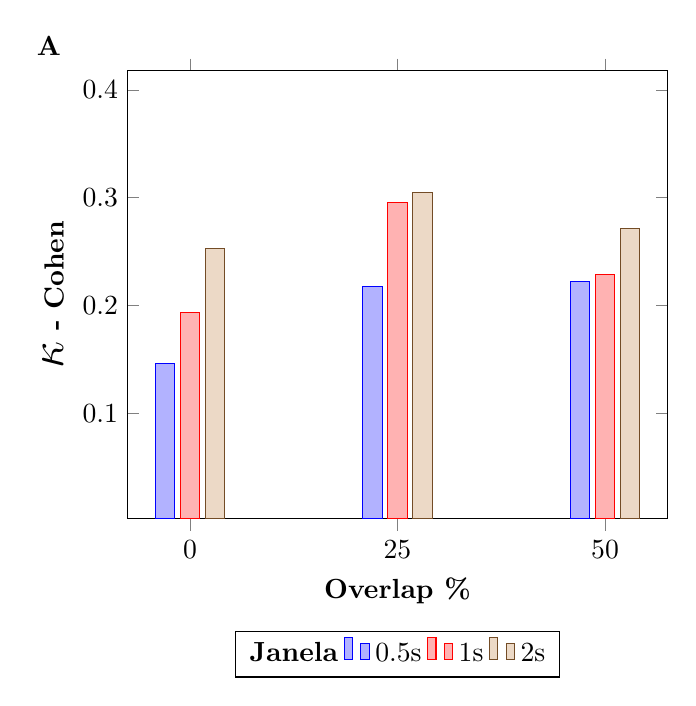
\begin{tikzpicture}
\begin{axis}[ybar,
ylabel={\textbf{{\LARGE $\kappa$} - Cohen}},
symbolic x coords={0,25,50},
enlargelimits=0.15,
bar width=7pt,
xlabel=\textbf{{Overlap \%}},
scale=1,
ymin=0.05,
ymax=0.37,
xtick=data,
legend style={at={(0.5,-0.25)},anchor=north,legend columns=-1},
]
\addlegendimage{empty legend}
\addlegendentry[]{\textbf{Janela}  }


\addplot coordinates{
	(0,0.145756921970514)
	(25,0.217953198653199)
	(50,0.222418529316488)
	
};
\addlegendentry{0.5s}
\addplot coordinates {
	(0,0.193445731381201)
	(25,0.295532180595581)
	(50,0.228335707502374)
};
\addlegendentry{1s}
\addplot coordinates {
	(0,0.253022486772487)
	(25,0.305006613756614)
	(50,0.271798941798942)
};
\addlegendentry{2s}

\end{axis}
\node[] at (-1,6) {\textbf{A}};
\end{tikzpicture}
	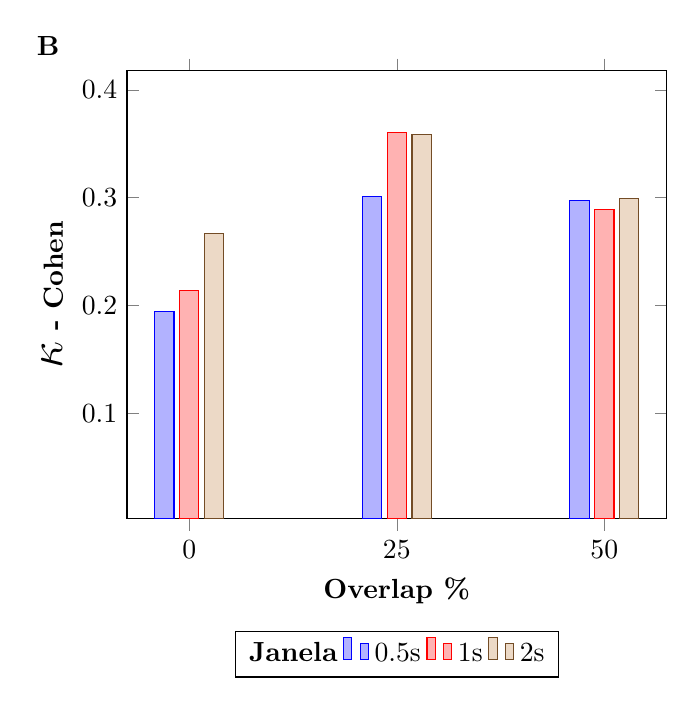
\begin{tikzpicture}
\begin{axis}[ybar,
ylabel={\textbf{{\LARGE $\kappa$} - Cohen}},
symbolic x coords={0,25,50},
enlargelimits=0.15,
bar width=7pt,
xlabel=\textbf{{Overlap \%}},
scale=1,
ymin=0.05,
ymax=0.37,
xtick=data,
legend style={at={(0.5,-0.25)},anchor=north,legend columns=-1},
]

\addlegendimage{empty legend}
\addlegendentry[]{\textbf{Janela}  }

\addplot coordinates{
	(0,0.194592780487009)
	(25,0.301151008868141)
	(50,0.297452810791095)
	
};
\addlegendentry{0.5s}
\addplot coordinates {
	(0,0.213851347718643)
	(25,0.360070705941324)
	(50,0.288910829755114)
};
\addlegendentry{1s}
\addplot coordinates {
	(0,0.2669239009365)
	(25,0.358554160497779)
	(50,0.299020891771033)
};
\addlegendentry{2s}
\end{axis}
\node[] at (-1,6) {\textbf{B}};
\end{tikzpicture}
\end{figure}
\subsection{Classificadores}
Na figura \ref{fig:ClassPerf} podemos observar que por uma margem significativa o classificador com a melhor performance foi o  \ac{L-SVM}. As redes neurais (\acs{ANN-2} e \acs{ANN-3} tiveram performances medianas junto com o \ac{C-SVM}.
 A pior performance por uma margem significativa foi do \ac{F-SVM} em que o parâmetro $K$ do kernel teve um impacto negativo na generaliza\c{c}\~ao do classificador. 
\begin{figure}[h]
	\caption{Performance m\'edia dos classificadores utilizados}
	\label{fig:ClassPerf}
	\centering
	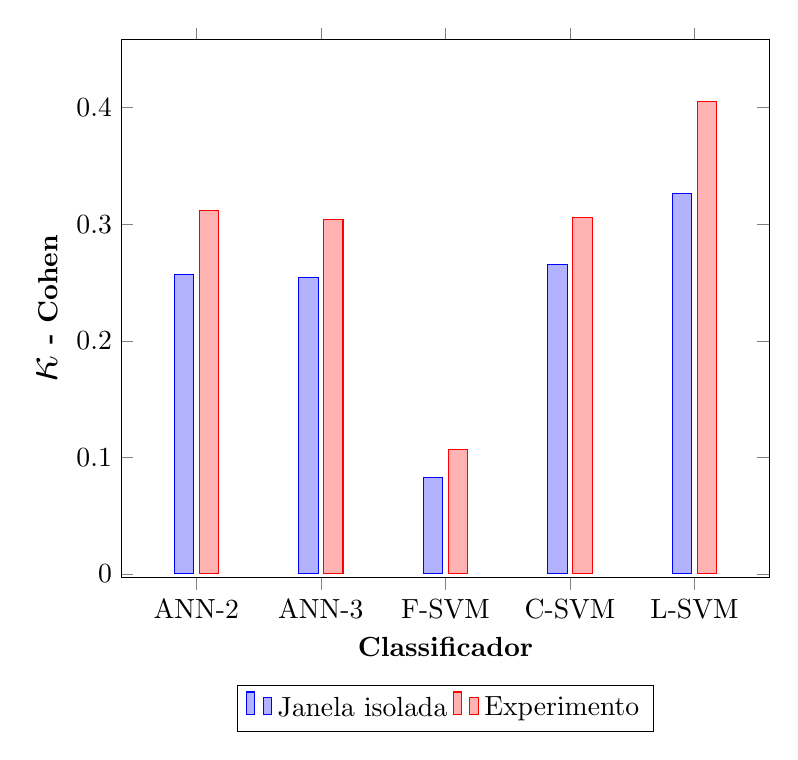
\begin{tikzpicture}
\begin{axis}[ybar,
ylabel={\textbf{{\LARGE $\kappa$} - Cohen}},
symbolic x coords={ANN-2,ANN-3,F-SVM,C-SVM,L-SVM},
enlargelimits=0.15,
bar width=7pt,
xlabel={\textbf{Classificador}},
xtick=data,
legend style={at={(0.5,-0.2)},anchor=north,legend columns=-1},
scale=1.2,
ymin=0.05,
]
\addplot coordinates {
	(ANN-2,0.256710322461084)
	(ANN-3,0.253969286000733)
	(F-SVM,0.08251886405747)
	(C-SVM,0.265203892414323)
	(L-SVM,0.32674780825939)
};
\addplot coordinates {
	(ANN-2,0.311612621296827)
	(ANN-3,0.304360005958168)
	(F-SVM,0.106615596193986)
	(C-SVM,0.305949166653495)
	(L-SVM,0.405089519212324)
};
\legend{Janela isolada,Experimento}
\end{axis}
\end{tikzpicture}
\end{figure}
\subsection{Fun\c{c}\~oes de extra\c{c}\~ao vs Janela de Amostragem}
A figura \ref{fig:PSDPerf} sugere que com o aumento da janela de amostragem a performance melhora igualmente para os \ac{PWelch} e \ac{PMTM} sendo que o desempenho do \ac{PMTM} foi ligeiramente maior. O \ac{PSDp} teve claramente a pior performance isso \'e poss\'ivelmente devido \`a sua falta de capacidade de lidar com ru\'idos. 
\begin{figure}[h]
	\caption{Performance m\'edia das Fun\c{c}\~oes de extra\c{c}\~ao utilizadas vs Janela de amostragem}
	\label{fig:PSDPerf}
	\centering
	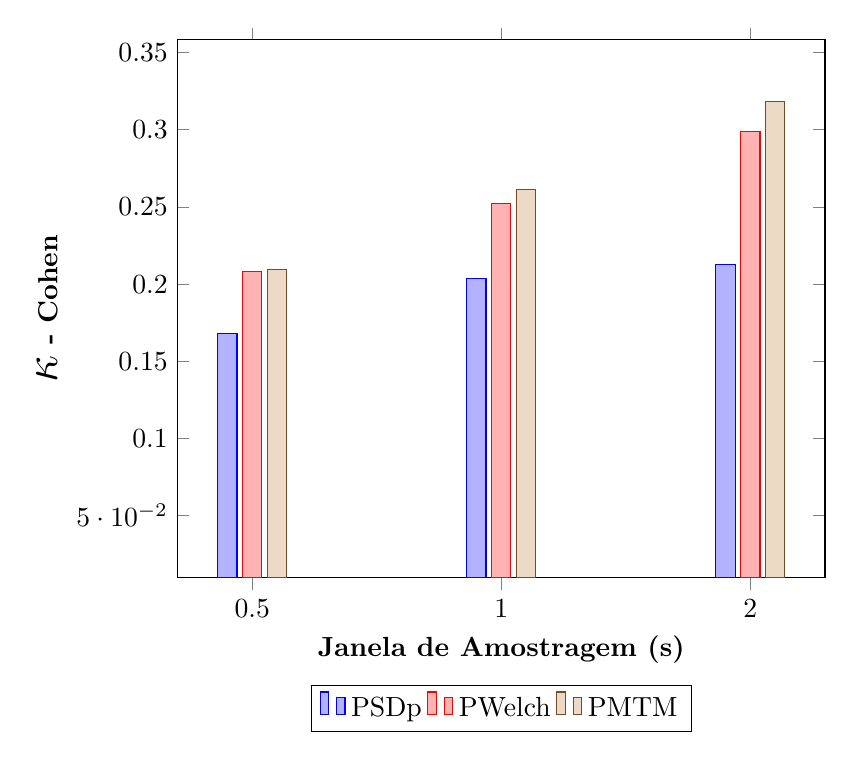
\begin{tikzpicture}
\begin{axis}[ybar,
ylabel={\textbf{{\LARGE $\kappa$} - Cohen}},
symbolic x coords={0.5,1,2},
enlargelimits=0.15,
bar width=7pt,
xlabel={\textbf{Janela de Amostragem (s)}},
xtick=data,
legend style={at={(0.5,-0.2)},anchor=north,legend columns=-1},
scale=1.2,
ymin=0.05,
]

\addplot coordinates {

	(0.5,0.168200019315786)
	(1,0.20381375312512)
	(2,0.212802028218695)

};
\addlegendentry[]{PSDp}
\addplot coordinates {
	(0.5,0.208379846569074)
	(1,0.252435974315611)
	(2,0.298970458553792)
};
\addlegendentry[]{PWelch}
\addplot coordinates {
	(0.5,0.209548784055341)
	(1,0.261063892038425)
	(2,0.318055555555556)
};
\addlegendentry[]{PMTM}
\end{axis}
\end{tikzpicture}
\end{figure}
\section{Melhores Performances}
\par Pode-se observar nas tabelas abaixo a preval\^encia do \ac{L-SVM} nas melhores posi\c{c}\~oes entre os classificadores e do \ac{PMTM} nas fun\c{c}\~oes de extra\c{c}\~aos. Na performance utilizando o intervalo completo e na performance de janela de amostragem de at\'e 2 segundos o melhor overlap foi de 25\% enquanto para a performance de at\'e 0.5 segundos o melhor overlap foi o de 50\%.
\begin{table}[h!]
	\centering
	\caption{Melhores performances na m\'etrica do experimento}
	\begin{tabularx}{\textwidth}{c|c|c|c|c|c|c|c|c}		
		\hline\hline
		Pos&$\kappa_1$ &$\text{ACC}_1$&$\kappa_2$&$\text{ACC}_2$&Janela& Overlap&Fun\c{c}\~ao&Classificador  \\ \hline 
		$1^{\underline{o}}$&0.422&71.14\%&0.526&76.32\%&2s&25\%&PWelch&\acs{L-SVM} \\ \hline 
		$2^{\underline{o}}$&0.426&71.35\%&0.512&75.62\%&2s&25\%&PMTM&L-SVM \\ \hline
		$3^{\underline{o}}$&0.421&71.06\%&0.491&74.58\%&2s&25\%&PMTM&\acs{ANN-3} \\ \hline
		$4^{\underline{o}}$&0.407&70.36\%&0.490&74.51\%&1s&25\%&PMTM&L-SVM \\ \hline
		$5^{\underline{o}}$&0.402&70.11\%&0.484&74.23\%&1s&25\%&PMTM&\ac{ANN-2} \\ \hline
	\end{tabularx}
	\label{Tab:melhoresKappaFull}
\end{table}

\begin{table}[h!]
	\centering
	\caption{Melhores performances por Janela de amostragem de at\'e 2s}
	\begin{tabularx}{\textwidth}{c|c|c|c|c|c|c|c|c}		
		\hline\hline
		Pos&$\kappa_1$ &$\text{ACC}_1$&$\kappa_2$&$\text{ACC}_2$&Janela& Overlap&Fun\c{c}\~ao&Classificador  \\ \hline
		$1^{\underline{o}}$&0.426&71.35\%&0.512&75.62\%&2s&25\%&PMTM&L-SVM \\ \hline 
		$2^{\underline{o}}$&0.422&71.14\%&0.526&76.32\%&2s&25\%&PWelch&L-SVM\\ \hline
		$3^{\underline{o}}$&0.421&71.07\%&0.452&72.61\%&2s&0\%&PMTM&L-SVM \\ \hline
		$4^{\underline{o}}$&0.421&71.06\%&0.491&74.58\%&2s&25\%&PMTM&ANN-3 \\ \hline
		$5^{\underline{o}}$&0.418&70.95\%&0.466&73.33\%&2s&50\%&PMTM&L-SVM \\ \hline
	\end{tabularx}
	\label{Tab:melhoresKappa}
\end{table}

\begin{table}[h!]
	\centering
	\caption{Melhores performances por Janela de amostragem de at\'e 0.5s}
	\begin{tabularx}{\textwidth}{c|c|c|c|c|c|c|c|c}		
		\hline\hline
		Pos&$\kappa_1$ &$\text{ACC}_1$&$\kappa_2$&$\text{ACC}_2$&Janela& Overlap&Fun\c{c}\~ao&Classificador  \\ \hline
		$1^{\underline{o}}$&0.293&64.69\%&0.401&70.09\%&0.5s&	50\%&PMTM&L-SVM \\ \hline 
		$2^{\underline{o}}$&0.286&64.31\%&0.388&69.45\%&0.5s&	50\%&PWelch&L-SVM \\ \hline
		$3^{\underline{o}}$&0.284&64,21\%&0.399&69.98\%&0.5s&25\%&PMTM&L-SVM \\ \hline
		$4^{\underline{o}}$&0.280&64,01\%&0.397&69.88\%&0.5s&25\%&PWelch&L-SVM \\ \hline
		$5^{\underline{o}}$&0.275&63.78\%&0.391&69.57\%&0.5s&	25\%&PMTM&ANN-2 \\ \hline
	\end{tabularx}
	\label{Tab:melhoresKappa125}
\end{table}
